\documentclass[conference]{IEEEtran}
\IEEEoverridecommandlockouts
% The preceding line is only needed to identify funding in the first footnote. If that is unneeded, please comment it out.
\usepackage{cite}
\usepackage{amsmath,amssymb,amsfonts}
\usepackage{algorithmic}
\usepackage{graphicx}
\usepackage{textcomp}
\usepackage{xcolor}
\usepackage{placeins}
\usepackage[hidelinks]{hyperref}
\usepackage{float}
\usepackage{subcaption}
\def\BibTeX{{\rm B\kern-.05em{\sc i\kern-.025em b}\kern-.08em
    T\kern-.1667em\lower.7ex\hbox{E}\kern-.125emX}}
\begin{document}

\title{Redes Neurais Convolucionais}

\author{\IEEEauthorblockN{Arthur Abrahão Santos Barbosa}
\IEEEauthorblockA{\textit{Universidade Federal de Pernambuco} \\
\textit{Centro de Informática}\\
Pernambuco, Brasil \\
aasb2@cin.ufpe.br}
\and
\IEEEauthorblockN{Filipe Samuel da Silva}
\IEEEauthorblockA{\textit{Universidade Federal de Pernambuco} \\
\textit{Centro de Informática}\\
Pernambuco, Brasil \\
fss8@cin.ufpe.br}

}

\maketitle





\section{Objetivos}

\subsection{Objetivo Geral}

Desnvolver um Classificador Multiclasse que reconheça as imagens do dataset CIFAR100 \cite{dataset}. 
\subsection{Objetivos Específicos}
\begin{itemize}
\item Compreender a implementação de uma Rede Neural Convolucional
\item Demonstrar a Importância do Aprendizado Profundo e suas aplicações
\item Demonstrar a eficiência de três arquiteturas importantes para a história do Deep Learning
\end{itemize}
\section{Justificativa}
Este projeto foi escolhido com base no fato deste dataset ser bastante usado para testar redes neurais com imagens coloridas, 
e pelo fato de ter uma divisão bastante equilibrada dos dados.\cite{dataset}.


Sua função é verificar a qual das classes pertence uma imagem de tamanho 32x32.

\section{Base de Dados}

O dataset usado durante o projeto é o CIFAR-100.
Ele tem 100 classes contendo 600 imagens cada, totalizando 60.000 imagens.
Das 600 imagens que cada classe possui 100 delas são separadas para teste e 500 delas para treino.
As 100 classes do dataset estão agrupadas em 20 super classes do seguinte modo\cite{dataset}:

\begin{itemize}
    \item \textbf{aquatic mammals:} 	beaver, dolphin, otter, seal, whale
    \item \textbf{fish:} 	aquarium fish, flatfish, ray, shark, trout
    \item \textbf{flowers:} 	orchids, poppies, roses, sunflowers, tulips
    \item \textbf{food containers:} 	bottles, bowls, cans, cups, plates
    \item \textbf{fruit and vegetables:} 	apples, mushrooms, oranges, pears, sweet peppers
    \item \textbf{household electrical devices:} 	clock, computer keyboard, lamp, telephone, television
    \item \textbf{household furniture:} 	bed, chair, couch, table, wardrobe
    \item \textbf{insects:} 	bee, beetle, butterfly, caterpillar, cockroach
    \item \textbf{large carnivores:} 	bear, leopard, lion, tiger, wolf
    \item \textbf{large man-made outdoor things:} 	bridge, castle, house, road, skyscraper
    \item \textbf{large natural outdoor scenes:} 	cloud, forest, mountain, plain, sea
    \item \textbf{large omnivores and herbivores:} 	camel, cattle, chimpanzee, elephant, kangaroo
    \item \textbf{medium-sized mammals:} 	fox, porcupine, possum, raccoon, skunk
    \item \textbf{non-insect invertebrates:} 	crab, lobster, snail, spider, worm
    \item \textbf{people:} 	baby, boy, girl, man, woman
    \item \textbf{reptiles:} 	crocodile, dinosaur, lizard, snake, turtle
    \item \textbf{small mammals:} 	hamster, mouse, rabbit, shrew, squirrel
    \item \textbf{trees:} 	maple, oak, palm, pine, willow
    \item \textbf{vehicles 1:} 	bicycle, bus, motorcycle, pickup truck, train
    \item \textbf{vehicles 2:}	lawn-mower, rocket, streetcar, tank, tractor

\end{itemize}
\cite{dataset}


\section{Análise Exploratória dos Dados}

\subsection{Quantidade de Imagens Por Classes}

Tanto o dataset de teste quanto o de treino são bastante equilibrados,
possuindo a mesma quantidade de imagens para cada classe:


\subsection{Descrição Estatística dos dados}

Porque os dados trabalhados são imagens em vez de tabelas,
é mais difícil descrevê-las estatisticamente.
Portanto as descrevemos do seguinte modo:

\subsubsection{Média das Imagens por Classe}

Um método possível de analisar as imagens estatisticamente
é cálcular o valor médio por pixel, e deste modo conseguir uma imagem média que
representaria a classe.

\begin{itemize}
\item Média da Imagens Não Normalizadas
\end{itemize}

\begin{figure}[H]
\centerline{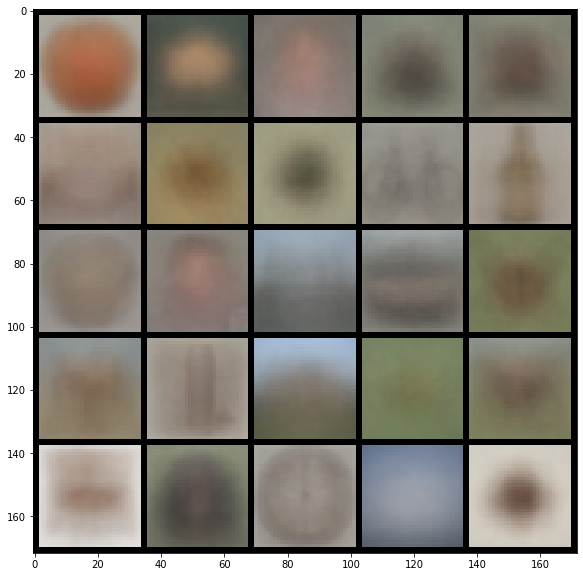
\includegraphics[width=0.4\textwidth]{Images/img_mean1.png}}
\caption{\label{fig:img_mean1}Da esquerda para a direita, de cima para a baixo: apple, aquarium\_fish, baby, bear, beaver, bed, bee, beetle, bicycle, bottle, bowl, boy, bridge, bus, butterfly, camel, can, castle, caterpillar, cattle, chair, chimpanzee, clock, cloud, cockroach}
\end{figure}

\begin{figure}[H]
\centerline{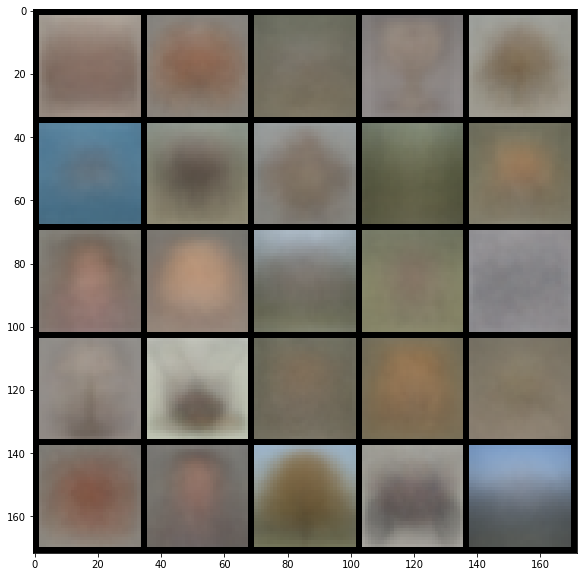
\includegraphics[width=0.4\textwidth]{Images/img_mean2.png}}
\caption{\label{fig:img_mean2}Da esquerda para a direita, de cima para a baixo: couch, crab, crocodile, cup, dinosaur, dolphin, elephant, flatfish, forest, fox, girl, hamster, house, kangaroo, keyboard, lamp, lawn\_mower, leopard, lion, lizard, lobster, man, maple\_tree, motorcycle, mountain}
\end{figure}

\begin{figure}[H]
\centerline{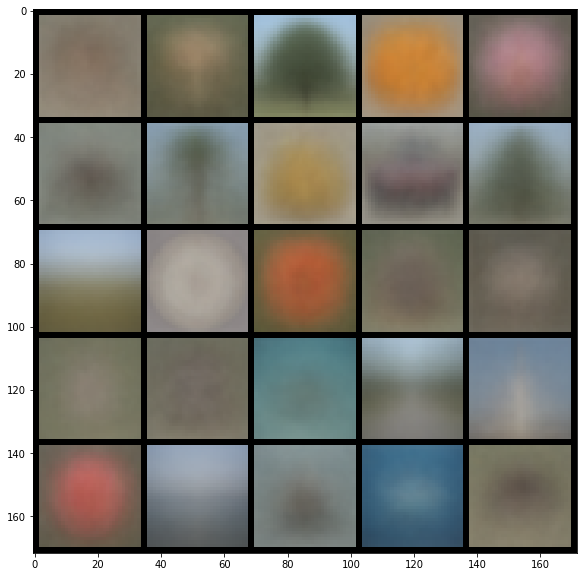
\includegraphics[width=0.4\textwidth]{Images/img_mean3.png}}
\caption{\label{fig:img_mean3}Da esquerda para a direita, de cima para a baixo: mouse, mushroom, oak\_tree, orange, orchid, otter, palm\_tree, pear, pickup\_truck, pine\_tree, plain, plate, poppy, porcupine, possum, rabbit, raccoon, ray, road, rocket, rose, sea, seal, shark, shrew}
\end{figure}

\begin{figure}[H]
\centerline{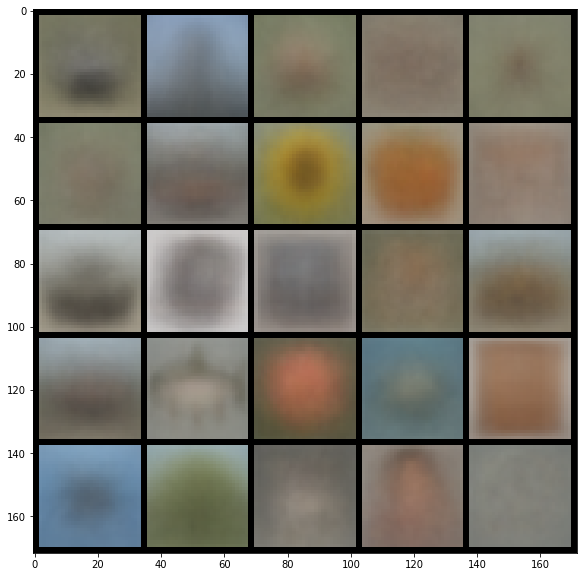
\includegraphics[width=0.4\textwidth]{Images/img_mean4.png}}
\caption{\label{fig:img_mean4}Da esquerda para a direita, de cima para a baixo: skunk, skyscraper, snail, snake, spider, squirrel, streetcar, sunflower, sweet\_pepper, table, tank, telephone, television, tiger, tractor, train, trout, tulip, turtle, wardrobe, whale, willow\_tree, wolf, woman, worm}
\end{figure}

\begin{itemize}
\item Média da Imagens Normalizadas
\end{itemize}

\begin{figure}[H]
\centerline{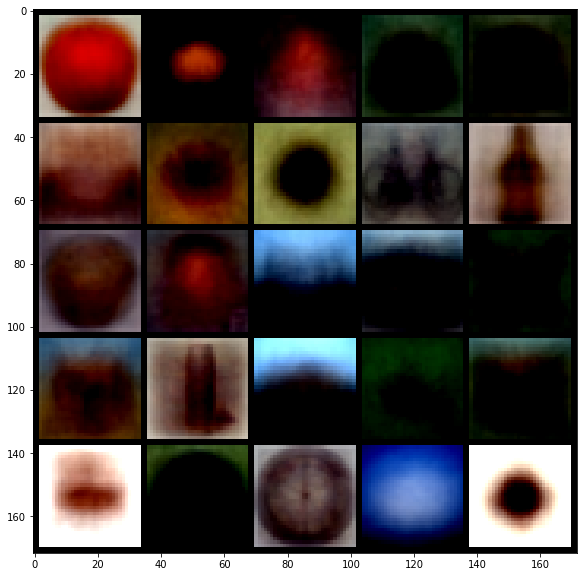
\includegraphics[width=0.4\textwidth]{Images/img_mean_norm1.png}}
\caption{\label{fig:img_mean_norm1}Da esquerda para a direita, de cima para a baixo: apple, aquarium\_fish, baby, bear, beaver, bed, bee, beetle, bicycle, bottle, bowl, boy, bridge, bus, butterfly, camel, can, castle, caterpillar, cattle, chair, chimpanzee, clock, cloud, cockroach}
\end{figure}

\begin{figure}[H]
\centerline{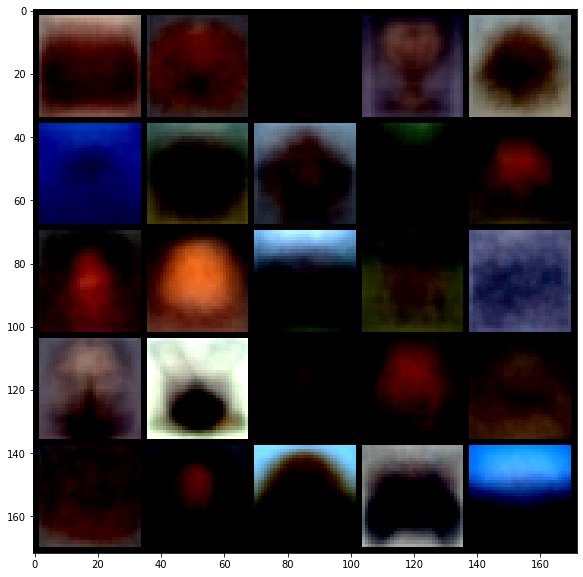
\includegraphics[width=0.4\textwidth]{Images/img_mean_norm2.png}}
\caption{\label{fig:img_mean_norm2}Da esquerda para a direita, de cima para a baixo: couch, crab, crocodile, cup, dinosaur, dolphin, elephant, flatfish, forest, fox, girl, hamster, house, kangaroo, keyboard, lamp, lawn\_mower, leopard, lion, lizard, lobster, man, maple\_tree, motorcycle, mountain}
\end{figure}

\begin{figure}[H]
\centerline{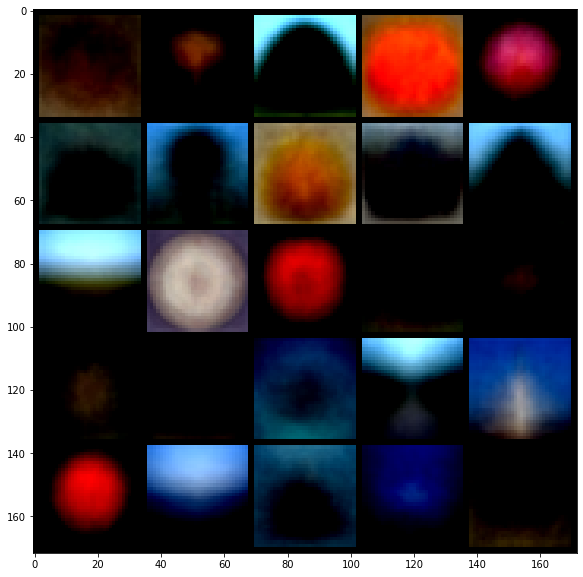
\includegraphics[width=0.4\textwidth]{Images/img_mean_norm3.png}}
\caption{\label{fig:img_mean_norm3}Da esquerda para a direita, de cima para a baixo: mouse, mushroom, oak\_tree, orange, orchid, otter, palm\_tree, pear, pickup\_truck, pine\_tree, plain, plate, poppy, porcupine, possum, rabbit, raccoon, ray, road, rocket, rose, sea, seal, shark, shrew}
\end{figure}

\begin{figure}[H]
\centerline{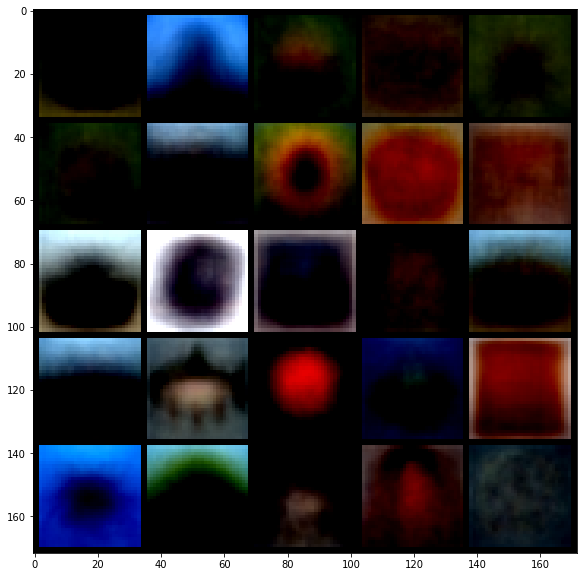
\includegraphics[width=0.4\textwidth]{Images/img_mean_norm4.png}}
\caption{\label{fig:img_mean_norm4}Da esquerda para a direita, de cima para a baixo: skunk, skyscraper, snail, snake, spider, squirrel, streetcar, sunflower, sweet\_pepper, table, tank, telephone, television, tiger, tractor, train, trout, tulip, turtle, wardrobe, whale, willow\_tree, wolf, woman, worm}
\end{figure}
    
%\subsection{Sobre o Projeto}
%Para montar o classificador foi necessário passar  pelas seguintes etapas:



\section{Sobre as Métricas Utilizadas}

\subsection{Precision}

Precision é a razão
    \begin{equation}
        \frac{A_c}{A_c + A_e}
    \end{equation}

    onde:

    \begin{itemize}
    \item $A_c$ é o número de amostras corretamente classificadas de uma determinada classe.
    \item $A_e$ é o número de amostras  erroneamente classificadas como sendo desta determinada classe.
    \end{itemize}

    Precision é intuitivamente a habilidade do classificador não marcar como pertencente a uma classe uma amostra que não pertence a esta. O melhor valor de Precision é 1 e o pior é zero.
    \cite{b7}
\subsection{Accuracy} 

Accuracy é a fração de amostras preditas corretamente, e é dada pela seguinte fórmula:

\begin{equation}
    \frac{\sum\limits_{1}^{n}A_c}{\sum\limits_{1}^{n}A_t}
\end{equation}




onde:
\begin{itemize}
    \item $n$ é o número de classes
    \item $A_c$ é o número de amostras corretamente classificadas de uma determinada classe.
    \item $A_t$ é o número de amostras que pertencem a uma determinada classe
\end{itemize}

\cite{b8}
\subsection{Recall-Score}
O Recall Score é a razão:

    \begin{equation}
        \frac{A_c}{A_t}
    \end{equation}
    onde:
    \begin{itemize}
        \item $A_c$ é o número de amostras classificadas corretamente de uma determinada classe
        \item $A_t$ é o número de amostras que pertencem a esta classe
    \end{itemize}
    O Recall Score é intuitivamente a habilidade do classificador de encontrar todas as amostras pertencentes a uma classe especifica. O melhor valor do Recall Score é 1 e o pior valor é 0.
    \cite{b6}

\subsection{F1-Score}
O F1 Score pode ser interpretado como a média ponderada da precisão e recall. O melhor valor que o  F1 score pode alcançar é 1, o pior é 0. A contribuição relativa da precisão e recall para o F1 score são iguais. A fórmula para o F1 score é:
\begin{equation}
    F1 = \frac{2\cdot(precision\cdot recall)}{precision + recall}
\end{equation}
\cite{b2}
\subsection{Confusion Matrix}
No caso de classificação multiclasse, uma confusion matrix é dividida em NxN categorias(onde N é o número de classes do problema), cada uma apresentando a quantidade de amostras que se encaixam nesta.
A diagonal do meio representa a quantidade de amostras classificadas corretamente e as demais seções da matriz demonstram o número de amostras classificados erroneamente, a quais classes eles pertencem e em quais classes eles foram classificados.

\cite{metrics}




\subsection{O Nosso Modelo}
O modelo que escolhemos não é tão robusto na quantidade de parâmetros, porém é inspirado em soluções modernas de redes convolucionais.
Possui quatro camadas convolucionais, além de Batch Normalization e DropOut, que são técnicas para evitar alguns problemas advindos do treinamento com o conjunto de treino e validação com o conjunto de teste. Além da camadas totalmente conectadas, para transformação dos parâmetros de saída das convoluções em valores das classes de saida do problema.

\subsection{LeNet}
Um modelo bem simples e que vem dos primórdios da estrutura de rede neural convolucional, proposto por Yann LeCun, em 1989, para lidar com a extração de características das imagens de entrada, aplicando os princípios de redes convolucionais, que são boas para obtenção de características, em dados que têm dependência espacial. 

\subsection{AlexNet}
Modelo mais moderno, porém já utilizado como base para geração de outros modelos. Possui uma estrutura bem robusta, porém sua grande sacada, é a idéia proposta pelo trio Krizhevsky, Sutskever e Hinton, que utilizou do grande poder das GPUs para realizar o treinamento das redes, com uma rede apropriada para se utilizar desse potencial de processamento.

\begin{figure}[h]
	\centerline{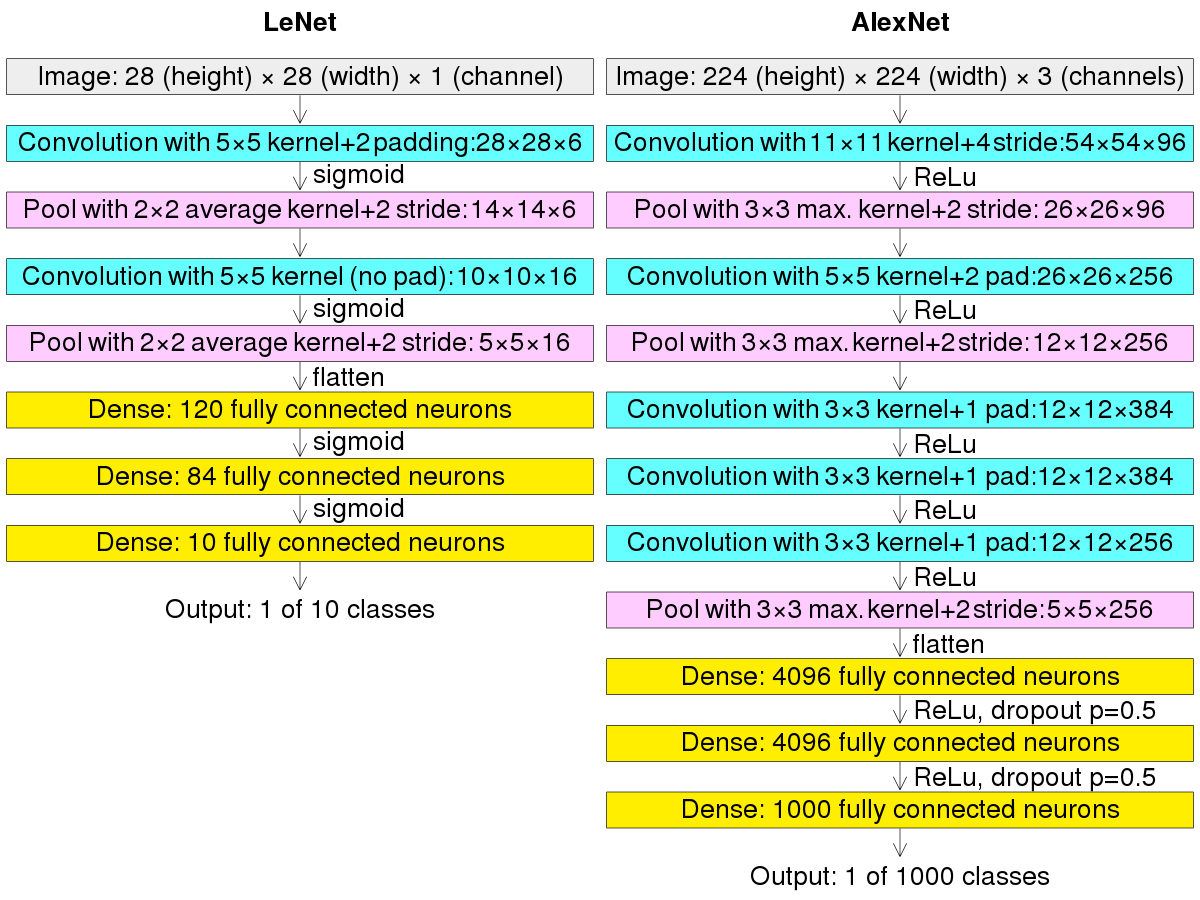
\includegraphics[width=8cm]{Images/Comparison_image_neural_networks.svg.png}}
	
	\caption{\label{fig:fig2}Diferença entre os modelos LeNet e AlexNet}
\end{figure}

Os Modelos da LeNet e AlexNet foram modificados de maneira a receber como entrada imagem de resolução 32x32, sem precisar de um resize. Outra modificação q se mostrou interessante foi a aplicação da Relu ao invés da Sigmoid.


\section{Experimentos}

%\subsection{Experimentos Iniciais}

\subsection{CIFAR10}
Foram realizados experimentos com o CIFAR10 que é como um subconjunto de classes pertencentes ao CIFAR100, possui 10 categorias de saída, e é util para fazer uma avaliação rápida e com pouco treinamento, garantindo ainda assim, boa performance dos modelos.

\subsection{Similaridade de Pixel}

Baseado na abordagem do fastai \cite{howard2020deep}
iremos criar um modelo básico que não utiliza aprendizado de máquina, 
para ter uma precisão como base para verificar o desempenho dos próximos modelos.
Esse método basicamente cálcula uma imagem média para cada classe do conjunto de treino, 
esta imagem média é basicamente uma imagem formada pela média de cada pixel das imagens de uma classe.

Para fazer a predição esta arquitetura basicamente cálcula a distância de uma imagem a imagem média,
e escolhe a classe com a menor distância.
Podemos usar o erro quadrático médio ou o valor absoluto das diferenças como valor da distância total entre uma imagem e a média da sua classe.

Porém, ao contrário da abordagem original do fastai para o dataset mnist com apenas duas classes com imagens em preto e branco, 
que teve uma 'accuracy' razoável com este método, temos que a 'accuracy' que tivemos com o CIFAR 100 que possui muito mais classes,
e imagens coloridas, não é melhor do que selecionarmos uma classe ao acaso.

\subsection{Treinando os Modelos}
Os dados do dataset que foram separados, agora serão usados para o treinamento e avaliação da performance das redes neurais.
Para realizar o treino os dados foram separados em batchs, e todos os três modelos foram treinados durante 50 épocas, para que houvesse um período de aprendizagem razoável de acordo com o tamanho das redes.
A cada época de treino e alguns batchs foram selecionados para mostrar a o valor da função loss, e mostrar a evolução do treinamento em diferentes épocas.

Os desempenhos da nossa rede, foram melhores que as duas outras, em 50 épocas de treinamento:
O nosso modelo, garantiu a acurácia

\begin{itemize}
	\item Nosso: de $\frac{5520}{10000}$ = 55.2\%
	\item LeNet: 1\%
	\item AlexNet: de ${4906 \over 10000}$ = 49.059999999999995\%
\end{itemize}

E um exemplo do desempenho do nosso modelo para cada classe do dataset:
\begin{figure}[h]
	\centerline{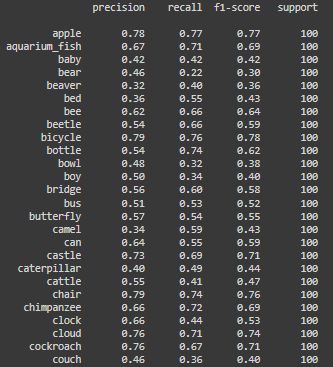
\includegraphics[width=8cm]{Images/treinamento2.png}}
	
	\caption{\label{fig:fig2}Desempenho 50 Épocas}
\end{figure}


\subsection{Apenas um Epoch}
Para o treinamento com apenas uma época, nós restauramos o modelo ao estado sem treinamento, e determinamos o num epochs como 1. Esse tipo de treinamento serve para avaliar a perfomance inicial do modelo ao ser corrigido pelas funções de perda.

O nosso modelo, também garantiu melhor desempenho com apenas uma época, com acurácia de 14.85\%, enquanto a acurácia da AlexNet foi de 14.85\%, já a LeNet apenas 1\%.

\subsection{Limitando os Dados}
O treinamento com limitação de dados também é uma boa opção para avaliar a capacidade das redes em aprender com poucos exemplos.
É possível perceber que os desempenhos de todas as redes acaba caindo, pois existe um princípio, de que, quanto mais exemplos de todas as classes você tiver, mais preciso e mais acurado ele tenderá a ser. Ou seja, ele irá aprender mais sobre aquelas classes.
Foi utilizado então, como objetivo de atingir esse experimento, a utilização dos dados de treinamento como dados de teste, e os dados de teste serviram como treinamento.
Nesse caso, apesar da perda de desempenho, nosso modelo teve a performance de 30.194\%, a AlexNet de 19.054\% e a LeNet de 1\%

\subsection{Sem Normalização e sem Data Augmentation}
Por último, foi realizado o treinamento sem normalização. A normalização é uma estratégia para que o treinamento seja realizado mais rapidamente, e para evitar alguns problemas que podem surgir nas métricas das funções de erro.
Os desempenhos sem normalização foram um pouco menores, o que nos mostra que essa estratégia é realmente útil para se aplicar nos treinamentos da rede.
A nossa rede obteve, 49.76\% de acurácia, a AlexNet 42.1\% e a LeNet apenas 0.67\%

Esse desempenho da LeNet nos levou a uma modificação.





%\subsection{Modelos Pré-Treinados}

\section{Análise dos Resultados}
\subsection{LeNet com Relu}
Nós nos deparamos com um problema, a rede LeNet com a função sigmoid estava tendo resultados muito abaixo, comparado as demais, redes. Abaixo até mesmo considerando a complexidade do tamanho da rede. Portanto, modificamos a rede para uma função ReLu no lugar da sigmoid, e obtivemos bom resultado. Temos que a sua acurácia aumentou para 33.75\%. Isso mostra a modernidade da ReLU, como função de ativação.
\subsection{Desempenho da rede com os dados ruidosos}
Para avaliar o desempenho das redes, aplicamos um ruido gaussiano nas imagens de teste, e testamos a acurácia da rede, mesmo após a aplicação do filtro que gerou o ruido e tivemos as acurácias de 17.97\% do nosso modelo convolucional, 28.02\% a LeNet com Relu e 8.18\% a AlexNet

\begin{figure}[h]
	\centerline{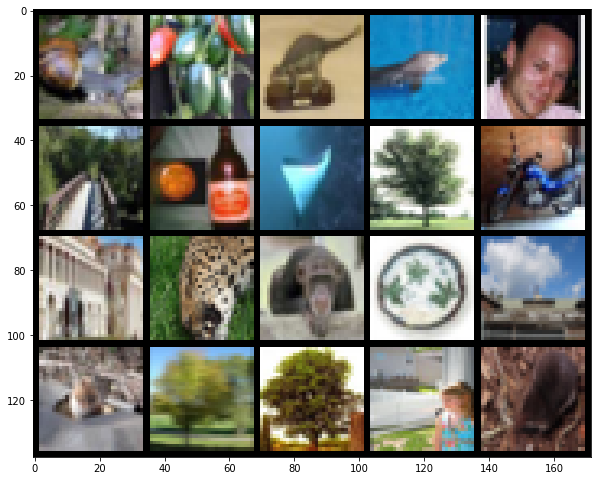
\includegraphics[width=8cm]{Images/imagensnoised.png}}
	
	\caption{\label{fig:fig2}Imagens Ruidosas}
\end{figure}


\section{Conclusões e Discussões}
Podemos observar que, para determinados problemas, existem soluções variadas e, geralmente, temos que obter dados específicos do problema para construir uma solução viável. Isso se aplica as redes neurais em geral, e as redes convolucionais, especificamente. Vemos que o tamanho do modelo, não implica em eficácia, e também que as diferentes variações dos modelos, geram novas soluções e melhores. Apesar da grande proposta das redes profundas, lidar com a idéia da máquina extraindo todas as caracteristicas e funcionando com um sistema que apenas inserimos os dados como entrada, vemos que, as redes para resolver diferentes problemas, possuem diferentes tamanhos e formatos, baseados em considerações particulares das condições do problema analisado, ou seja, vemos muitos modelos adaptados aos diferentes tipos e formatos de dados, em contraste com um modelo mais abstrato e generalista. (Com destaque, para algumas propostas modernas de modelos generalistas, que estão atualmente implementados) Apesar disso, a quantidade de aplicações das redes neurais e a facilidade de adaptação das redes para resolver vários tipos de problemas, é o que garante a grande capacidade dessas redes em realmente aprender diversos tipos de questões abstratas, o que significa que elas podem realmente, aprender sobre os dados.

\bibliography{mybib}
\nocite{*}
\bibliographystyle{IEEEtran}
\end{document}
